\documentclass[12pt,a4paper]{article}
\usepackage[top=1in,bottom=1in,left=1.25in,right=1in]{geometry}
\usepackage{mathptmx}
\usepackage[T1]{fontenc}
\usepackage{xcolor}
\usepackage{array}
\usepackage{longtable}
\usepackage{colortbl}
\usepackage{enumitem}
\usepackage{setspace}
\usepackage{fancyhdr}
\usepackage{titlesec}
\usepackage[most]{tcolorbox}
\usepackage{microtype}
\usepackage{needspace}
\usepackage{amsmath}
\usepackage{tikz}
\usetikzlibrary{positioning,arrows.meta,fit,backgrounds,calc}
\usepackage[hidelinks]{hyperref}
\usepackage{tocloft}
\renewcommand{\cftsecleader}{\cftdotfill{\cftdotsep}}
\setlength{\cftbeforesecskip}{3pt}

\definecolor{navy}{HTML}{000000}
\definecolor{purp}{HTML}{000000}
\definecolor{dred}{HTML}{000000}
\definecolor{azure}{HTML}{000000}
\definecolor{gbox}{HTML}{EAF2FA}
\definecolor{gborder}{HTML}{9AA5B1}
\definecolor{gtext}{HTML}{404040}
\definecolor{ghead}{HTML}{F2F2F2}
\definecolor{covergrey}{HTML}{767171}
\definecolor{tdark}{HTML}{3A3A3A}
\definecolor{tblue}{HTML}{1F3864}

\setstretch{1.4}
\setlength{\parindent}{0pt}
\setlength{\parskip}{6pt}
\pagestyle{empty}
\setlist{nosep}
\setlist[itemize]{leftmargin=2.2em,itemsep=2pt}

% Headings
\titleformat{\section}{\bfseries\fontsize{14}{17}\selectfont\color{purp}}{\thesection.}{0.3em}{}
\titleformat{\subsection}{\bfseries\large\color{navy}}{\thesubsection}{0.4em}{}
\titlespacing*{\section}{0pt}{14pt}{6pt}
\titlespacing*{\subsection}{0pt}{10pt}{4pt}
\newcommand{\redsec}[1]{\par\vspace{8pt}\addcontentsline{toc}{section}{#1}{\centering\bfseries\fontsize{14}{17}\selectfont #1\par}\vspace{2pt}\nopagebreak}
\newcommand{\purpsec}[1]{\par\vspace{8pt}\addcontentsline{toc}{section}{#1}{\centering\bfseries\fontsize{14}{17}\selectfont #1\par}\vspace{2pt}\nopagebreak}
\newcommand{\dredrule}{}
\newcommand{\bluesub}[1]{\par\vspace{4pt}\addcontentsline{toc}{subsection}{#1}{\bfseries #1\par}\nopagebreak}
\newcommand{\navysub}[1]{\par\vspace{4pt}\addcontentsline{toc}{subsection}{#1}{\bfseries #1\par}\nopagebreak}
\newcommand{\purpsub}[1]{\par\vspace{3pt}\addcontentsline{toc}{subsection}{#1}{\bfseries #1\par}\nopagebreak}

% Guideline box
\newtcolorbox{guide}[1]{enhanced,colback=gbox,colframe=gborder,boxrule=0.5pt,arc=0pt,
  left=6pt,right=6pt,top=3pt,bottom=3pt,
  fontupper=\itshape\small\color{gtext},before upper={\setstretch{1.15}\setlength{\parskip}{3pt}},
  title={\color{navy}\bfseries\upshape #1},coltitle=navy,colbacktitle=gbox,
  attach title to upper={\par},fonttitle=\small}

\setlength{\LTpre}{0pt}\setlength{\LTpost}{0pt}\setlength{\LTleft}{0pt}\setlength{\LTright}{0pt}

\begin{document}

% ---------------- COVER ----------------
\thispagestyle{empty}
\begin{tikzpicture}[remember picture,overlay]\draw[line width=2.5pt] ([shift={(1.5cm,1.5cm)}]current page.south west) rectangle ([shift={(-1.5cm,-1.5cm)}]current page.north east);\end{tikzpicture}
\begin{center}
\vspace*{0.6cm}
{\bfseries\fontsize{14}{17}\selectfont Department of Information Science \& Engineering}\\[3.2cm]
{\itshape\color{gtext}\Large Artificial Intelligence and Machine Learning}\\[0.5cm]
{\Large IS353IA}\\[1.1cm]
\end{center}

\noindent\fbox{\parbox{\dimexpr\linewidth-2\fboxsep-2\fboxrule\relax}{\centering\vspace{6pt}
{\bfseries\LARGE PROJECT SYNOPSIS}\\[4pt]
{\small Lab -- Part B}\vspace{8pt}}}\\[-1pt]
\renewcommand{\arraystretch}{1.75}
\setlength{\parskip}{0pt}
{\setlength{\fboxrule}{0.4pt}\noindent\hspace{-0pt}\begin{tabular}{|>{\raggedright\arraybackslash\bfseries\small}p{\dimexpr0.31\linewidth-12.4pt\relax}|p{\dimexpr0.69\linewidth-12.8pt\relax}|}
\hline
Title of Project: & {\hyphenpenalty=10000 \exhyphenpenalty=10000 A Sufficiency-Calibrated Framework for Evidentiary \mbox{Abstention} in Retrieval-Augmented Generation} \\ \cline{2-2}
Team No.: & B206 \\ \cline{2-2}
Student Name(s): & Snehal Reddy Thadigotla\newline Sumukha Upadhyaya \\ \cline{2-2}
USN / Reg. No.: & 1RV24IS126\newline 1RV24IS130 \\ \cline{2-2}
Semester and Section: & Vth Semester, ISE -- B \\ \cline{2-2}
Lab Batch: & B2 \\ \cline{2-2}
Date of Submission: & 03 / 10 / 2026 \\ \hline
\end{tabular}}

\vspace{2.2cm}
\begin{center}{\itshape\color{gtext}\small Academic Year: 2026--27}\end{center}

\newpage
\pagestyle{fancy}
\fancyhf{}
\fancyhead[R]{\small Sufficiency-Calibrated Evidentiary Abstention in RAG}
\fancyfoot[C]{\small\thepage}
\renewcommand{\headrulewidth}{0.8pt}
\renewcommand{\footrulewidth}{0.8pt}
\setlength{\headheight}{14.5pt}
\pagenumbering{roman}
\setcounter{tocdepth}{1}
\setstretch{1.15}
{\centering\bfseries\fontsize{14}{17}\selectfont Table of Contents\par}
\vspace{6pt}
{\setlength{\parskip}{0pt}\renewcommand{\contentsname}{}\makeatletter\@starttoc{toc}\makeatother}
\vspace{14pt}
{\centering\bfseries\fontsize{14}{17}\selectfont List of Abbreviations\par}
\vspace{6pt}
\renewcommand{\arraystretch}{1.25}
\begin{longtable}{|>{\raggedright\arraybackslash\bfseries}p{0.20\linewidth}|>{\raggedright\arraybackslash}p{0.70\linewidth}|}
\hline
RAG & Retrieval-Augmented Generation \\ \hline
LLM & Large Language Model \\ \hline
NLI & Natural Language Inference \\ \hline
NQ & Natural Questions \\ \hline
DPR & Dense Passage Retrieval \\ \hline
MIPS & Maximum Inner-Product Search \\ \hline
FAISS & Facebook AI Similarity Search (vector search library) \\ \hline
MIL & Multiple-Instance Learning \\ \hline
MLP & Multilayer Perceptron \\ \hline
XGBoost & eXtreme Gradient Boosting \\ \hline
CDD & Context-Driven Decomposition \\ \hline
CDD-lite & One-pass, parallel variant of CDD used as a divergence signal \\ \hline
ECE & Expected Calibration Error \\ \hline
AUROC & Area Under the Receiver Operating Characteristic curve \\ \hline
MRR & Mean Reciprocal Rank \\ \hline
nDCG & Normalised Discounted Cumulative Gain \\ \hline
RAGAS & Retrieval-Augmented Generation Assessment (evaluation framework) \\ \hline
RQ & Research Question \\ \hline
\end{longtable}
\newpage
\pagenumbering{arabic}
\setcounter{page}{1}
\setstretch{1.4}

\purpsec{1. Abstract}
\dredrule
Retrieval-augmented generation (RAG) conditions a language model on passages returned by a dense retriever, but its failure modes are heterogeneous. Under evidence insufficiency, no retrieved passage entails the answer. Under knowledge conflict and temporal staleness, the retrieved evidence is fluent, topically relevant and wrong: contradicted by a peer passage, superseded by a later revision of the same document, or adversarially perturbed. Prompt-level abstention is poorly calibrated on the latter, and most selective-prediction gates collapse both failures into a single scalar confidence.

This project proposes a lightweight post-draft verification gate that renders a release-or-abstain decision. The generator first emits a short answer and one declarative statement. The gate then scores two orthogonal axes. \emph{Answerability} is a premise--hypothesis entailment check of the statement against each retrieved chunk, using a cross-encoder natural language inference (NLI) verifier with multiple-instance pooling. \emph{Evidence reliability} aggregates inter-passage contradiction, divergence between context-conditioned and parametric answers, entailment-score dispersion, and revision metadata that exposes superseded document versions. A fixed decision table maps the two calibrated scores to release, regeneration from the newest revision, or abstention.

Evaluation uses seven controlled evidence regimes (clean, missing, conflicting, stale-current, stale-only, adversarial and old-but-valid) over a 1.5-million-passage Wikipedia corpus with exact maximum-inner-product search. A two-encoder variant is contrasted with a single classifier over frozen verifier features, and both are compared against retrieval-score, zero-shot verifier, set-level verifier and large language model (LLM) judge baselines, using risk--coverage curves, expected calibration error, latency and cost. The expected outcome is a quantified answer to whether a cheap two-axis gate approaches costly judges, together with an explicit statement of what no text-only gate can establish.

\textbf{Keywords:} {\itshape Retrieval-Augmented Generation, Selective Prediction, Epistemic Abstention, Knowledge Conflict Detection, Temporal Staleness, Multiple-Instance Pooling, Confidence Calibration}

\newpage
\purpsec{2. Introduction}

\navysub{2.1 Background}
Retrieval-augmented generation (RAG) is now the standard way to ground a language model in external documents. A retriever fetches the passages most similar to a question and the model writes an answer from them. The risk moves into the retrieved text: if the passages are wrong, the model can repeat them.

Two failures need to be kept apart. The first is \emph{missing evidence}: nothing retrieved supports an answer. Work on sufficient context shows that models often answer anyway rather than abstain~[1]. The second is \emph{misleading evidence}: a retrieved passage reads fluently, matches the question, and is wrong. Small frozen models still answer 41.6\% of misleading-context questions even when told to abstain when unsure~[2], and standard RAG reaches only 15.0\% accuracy under a worst-case misconception-injection probe~[3].

In deployed systems, misleading evidence most often appears as \emph{context rot}. A document collection evolves, and superseded versions of a fact stay searchable next to the current one. Evaluation on a static test set measures a snapshot and cannot reveal this effect.

Recent work has built cheap detectors for parts of this problem. A small claim--evidence verifier with set-level aggregation beats a GPT-4o judge on synthetic refutations~[4]. Lightweight classifiers detect conflicts at low cost~[5]. Lightweight predictors beat prompt-based abstainers on risk--coverage curves~[6]. Answerability and correctness are known to be separate axes of abstention~[7]. What none of these covers together is a gate that scores answerability and reliability as two separate quantities, reasons across retrieved passages, and is tested on temporal conflicts under realistic retrieval.

\navysub{2.2 Problem Statement}
Existing abstention gates either test only whether evidence is present, or merge presence and trustworthiness into one score. They therefore cannot tell \emph{missing} from \emph{conflicting} from \emph{outdated} evidence, and they are rarely evaluated on stale document versions under realistic retrieval. This project asks whether a cheap, independently calibrated two-axis gate can decide when a RAG system should abstain, at useful risk--coverage and cost, compared with single-axis gates and large language-model judges.

\navysub{2.3 Motivation}
A RAG system that answers confidently from stale or contradicted evidence is worse than one that declines, because users cannot see the failure. Judge models that read the full context are accurate but expensive to run on every query. A gate that costs a fraction of that, and that explains \emph{why} it abstained, would let deployers choose an operating point between wrongly answering and needlessly refusing. Either result of this study is useful: if the cheap gate matches the judges, deployment cost falls; if it does not, we show where the gap lies.

\redsec{3. Literature Survey / Review of Related Work}
\dredrule

\navysub{3.1 Sufficiency and Abstention}
Joren et al.~[1] show that RAG models often answer when the context is insufficient. A Gemini~1.5~Pro autorater reaches 93.0\% accuracy at labelling sufficiency on 115 examples, and using it for selective generation raises the share of correct answers among those given by 2--10\%. Wagner~[7] shows that correctness and answerability are separate axes across five models of 2--14B parameters. A hidden-state probe reaches 0.69--0.77 AUROC at spotting unanswerable false-premise questions. Dong and Shinnou~[8] control risk in selective answering using confidence intervals. These works motivate the two-axis view, but none builds a retrieval-time gate that scores reliability on its own axis.

\navysub{3.2 Conflicting and Misleading Evidence}
Setiawan~[2] introduces the GRAB-RAG benchmark and finds that three small frozen models (3.8--8B parameters) still answer 41.6\% of misleading questions, with 63\% of those answers repeating the planted wrong entity. Its natural-language-inference verifier fails when the misleading passage agrees with the model's own memory, which is why our parametric-divergence signal is used as a one-sided warning only. Chen et al.~[3] introduce Context-Driven Decomposition (CDD), an inference-time diagnostic that elicits a contextual answer and a prior answer and isolates the conflicting premise. Under a worst-case misconception-injection probe, standard RAG reaches only 15.0\%. CDD needs several generation steps per query, which is why we use only a one-pass version of it. WikiContradict~[9] provides 253 human-annotated real contradictions from Wikipedia, which we use for conflicts between different documents.

\navysub{3.3 Cheap Verifiers and Detectors}
SURE-RAG~[4] scores claim--evidence pairs with a DeBERTa-v3-base model and aggregates them over the retrieved set, reaching 0.908 macro-F1 against 0.728 for a GPT-4o judge on synthetic multi-hop refutations. Its conflicts are entity, number and date swaps, it uses one fixed retriever, and it has no temporal metadata. ConflictRAG~[5] combines an embedding classifier with selective LLM refinement to reach 90.8\% accuracy at 62\% lower API cost, but resolves conflicts by source credibility rather than abstaining. SABER~[6] uses lightweight predictors, without fine-tuning the language model, to choose between trusting the model, trusting the context, accepting either, or abstaining. Its risk--coverage curve dominates prompt-based abstainers, but it handles a single passage on a static benchmark. MiniCheck~[10] shows that verifiers of 355M--770M parameters approach GPT-4 at checking claims against documents (74.7\% against 75.3\% balanced accuracy), and AlignScore~[11] shows that chunk-sized premises with sentence-sized claims work best. We reuse this machinery for the answerability axis.

\navysub{3.4 Temporal Question Answering}
SituatedQA~[12] is derived from Natural Questions and provides temporal questions with answer timelines over December-2018 and February-2021 Wikipedia dumps. The December-2018 dump is the same one used for the standard Dense Passage Retrieval corpus~[13], so stale and current versions of an article can be paired directly. We use it to build the stale-current, stale-only and old-but-valid conditions.

\navysub{3.5 Selective Prediction, Verification Granularity and Pooling}
Selective prediction formalises a model that may reject inputs: the risk--coverage trade-off was characterised by El-Yaniv and Wiener~[14], and Geifman and El-Yaniv~[15] showed how to choose a rejection threshold that meets a target risk with high probability for deep networks. We use this framework to compare gates and to set thresholds. On the verification side, Laban et al.~[16] found that natural language inference models trained on sentence-level premises fail on document-level inputs, and that splitting into sentences and aggregating pair scores adds about five points. AlignScore~[11] later showed that chunk-level premises with sentence-level claims work best, which fixes our unit choice. Chen et al.~[17] show that indexing at proposition level helps retrieval for unsupervised retrievers, but with a six-fold larger index, so we keep the standard 100-word passage as the retrieval unit and treat granularity as a verification choice. Finally, Ilse et al.~[18] cast bag-level prediction as multiple-instance learning with an attention-based, permutation-invariant pooling operator. Our pair bags are a multiple-instance problem, and mean-plus-max pooling is the baseline against which attention pooling is tested.

\navysub{3.6 Research Gap Summary}
\par\nopagebreak\noindent{\setstretch{1}\small\bfseries Table 3.1: Research gap summary}\par\nopagebreak\vspace{2pt}
\renewcommand{\arraystretch}{1.5}
\begin{longtable}{|>{\raggedright\arraybackslash\setlength{\parskip}{0pt}\setstretch{1}}p{0.17\linewidth}|>{\raggedright\arraybackslash\setlength{\parskip}{0pt}\setstretch{1}}p{0.27\linewidth}|>{\raggedright\arraybackslash\setlength{\parskip}{0pt}\setstretch{1}}p{0.46\linewidth}|}
\hline
\rowcolor{ghead}\bfseries Reference & \bfseries Key Contribution & \bfseries Limitation / Research Gap \\ \hline
Joren et al., 2024 [1] & Context-sufficiency autorater; selective generation & Single score; relies on a large LLM; no conflict or staleness axis \\ \hline
Setiawan, 2026 [2]; Chen et al., 2026 [3] & Misleading-context failure rates; CDD diagnostic & Prompt-based abstention fails; CDD needs several generation steps per query \\ \hline
Qiu et al., 2026 [4] & Cheap set-level verifier beats GPT-4o on synthetic conflicts & Synthetic edits, fixed retriever, no temporal metadata, no passage--passage reasoning \\ \hline
Wang et al., 2026 [5] & Cheap conflict detection with selective LLM refinement & Resolves by source credibility; does not abstain; no staleness \\ \hline
Zhu et al., 2026 [6] & Lightweight self-aware predictors, risk--coverage & One passage, static benchmark, no separate missing-vs-conflicting signal \\ \hline
Wagner, 2026 [7] & Answerability and correctness are separate axes & Shows the axes exist; builds no retrieval-time evidence gate \\ \hline
Geifman \& El-Yaniv, 2017 [15] & Threshold selection for target risk & Generic classifiers; no evidence-conflict or staleness signal \\ \hline
Laban et al., 2021 [16]; Zha et al., 2023 [11] & Granularity of NLI verification & Summarisation and factual-consistency settings; not multi-passage conflict under retrieval \\ \hline
\end{longtable}

\textbf{Gap:} No existing work combines a separate answerability score and a separate evidence-reliability score, reasons across the retrieved passages, and tests the result on stale document versions under realistic retrieval. This project addresses that gap.

\redsec{4. Objectives}
\dredrule
The primary objectives of this project are:
\begin{itemize}
\item To design a draft--verify--release pipeline in which a two-axis gate scores answerability and evidence reliability separately and maps them to release, resolve or abstain through a fixed decision table.
\item To implement two gate variants, one with separate fine-tuned verifier encoders per axis and one with a single classifier over frozen verifier features, to test whether separating the axes helps.
\item To construct seven controlled evidence conditions (clean, missing, conflicting, stale-current, stale-only, adversarial, old-but-valid) over a 1.5-million-passage Wikipedia corpus with exact vector search and query-time filtering.
\item To evaluate both variants against five baselines using decision risk, answer risk, risk--coverage curves, calibration and cost, and to measure how much version metadata and reranking change the result.
\end{itemize}

\navysub{4.1 Scope and Delimitations}
\begin{itemize}
\item\relax \emph{In scope:} one generator (Llama-3.1-8B-Instruct), two embedding models (bge-small and arctic-embed-m), seven evidence conditions, two gate variants, five baselines, and dense-only retrieval with a reranked arm on conditions C, D and F.
\item\relax \emph{Out of scope:} detecting false-premise questions, improving retrieval quality, and any claim that evidence is true. Retrieval is a controlled variable except where it is the experiment.
\item\relax \emph{Deferred to stretch goals:} the shared-encoder variant, a third embedding model, cross-construction-family transfer, hybrid BM25 retrieval, a second generator, and the full 21-million-passage corpus.
\end{itemize}

\redsec{5. Proposed Methodology}
\dredrule

\bluesub{5.1 System Architecture Overview}
The system is a pre-release check. A retriever returns the top 10 passages for a question, each with a revision timestamp and a document identifier. In parallel, the generator (Llama-3.1-8B-Instruct) writes a draft, consisting of a short answer and one declarative statement, and a second no-context answer used as a warning signal. The gate then decides whether the draft is released. Figure~5.1 summarises the flow.

\begin{figure}[t]
\centering
\resizebox{\linewidth}{!}{%
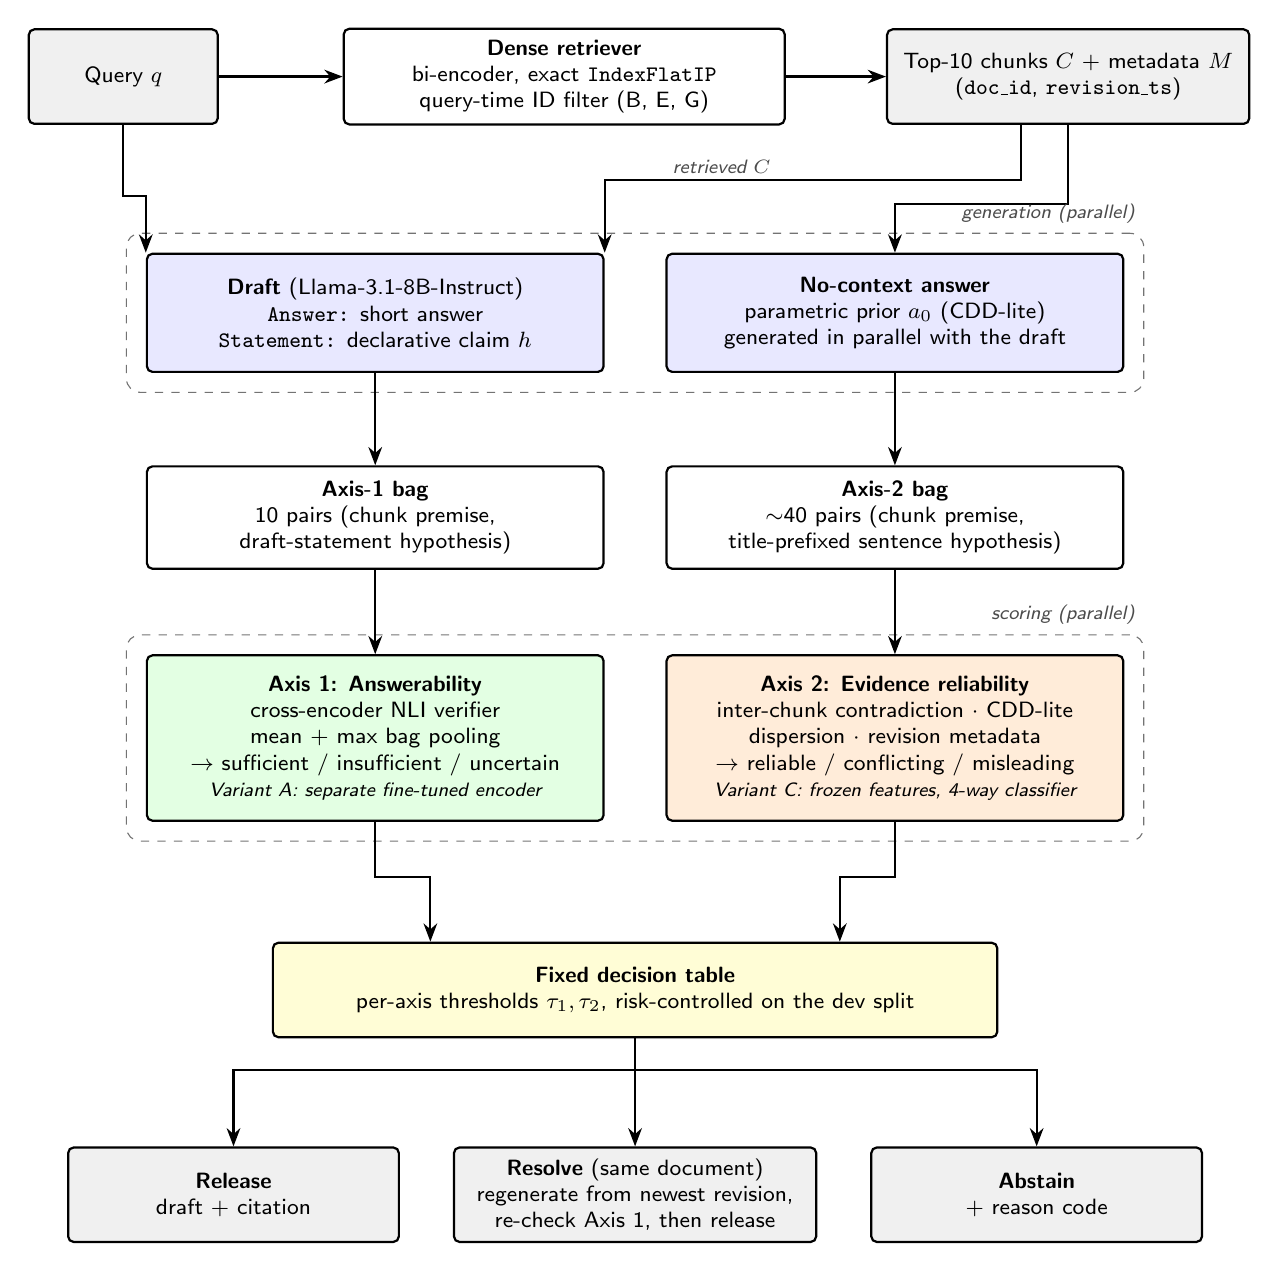
\begin{tikzpicture}[
  font=\sffamily\footnotesize,
  >=Stealth,
  box/.style={draw=black,rounded corners=2pt,thick,align=center,inner sep=4pt,fill=white},
  io/.style={box,fill=black!6},
  gen/.style={box,fill=blue!9},
  ax1/.style={box,fill=green!11},
  ax2/.style={box,fill=orange!15},
  outp/.style={box,fill=black!6},
  grp/.style={draw=black!55,dashed,rounded corners=5pt,inner sep=7pt},
  lbl/.style={font=\sffamily\scriptsize\itshape,black!70},
  arr/.style={->,thick}
]
% row 1: retrieval
\node[io,minimum width=2.4cm,minimum height=1.2cm] (q) at (0,0) {Query $q$};
\node[box,minimum width=5.6cm,minimum height=1.2cm] (ret) at (5.6,0) {\textbf{Dense retriever}\\bi-encoder, exact \texttt{IndexFlatIP}\\query-time ID filter (B, E, G)};
\node[io,minimum width=4.6cm,minimum height=1.2cm] (ctx) at (12.0,0) {Top-10 chunks $C$ + metadata $M$\\(\texttt{doc\_id}, \texttt{revision\_ts})};
\draw[arr] (q) -- (ret);
\draw[arr] (ret) -- (ctx);
% row 2: generation
\node[gen,minimum width=5.8cm,minimum height=1.5cm] (draft) at (3.2,-3.0) {\textbf{Draft} (Llama-3.1-8B-Instruct)\\\texttt{Answer:} short answer\\\texttt{Statement:} declarative claim $h$};
\node[gen,minimum width=5.8cm,minimum height=1.5cm] (nc) at (9.8,-3.0) {\textbf{No-context answer}\\parametric prior $a_0$ (CDD-lite)\\generated in parallel with the draft};
\draw[arr] (q.south) -- ++(0,-0.9) -| (draft.north west) ;
\draw[arr] (ctx.south) -- ++(0,-1.0) -| (nc.north);
\draw[arr] ([xshift=-0.6cm]ctx.south) -- ++(0,-0.7) -| (draft.north east);
\node[lbl] at (7.6,-1.15) {retrieved $C$};
% row 3: verification bags
\node[box,minimum width=5.8cm,minimum height=1.3cm] (b1) at (3.2,-5.6) {\textbf{Axis-1 bag}\\10 pairs (chunk premise,\\draft-statement hypothesis)};
\node[box,minimum width=5.8cm,minimum height=1.3cm] (b2) at (9.8,-5.6) {\textbf{Axis-2 bag}\\$\sim$40 pairs (chunk premise,\\title-prefixed sentence hypothesis)};
\draw[arr] (draft) -- (b1);
\draw[arr] (nc) -- (b2);
% row 4: axes
\node[ax1,minimum width=5.8cm,minimum height=2.1cm] (a1) at (3.2,-8.4) {\textbf{Axis 1: Answerability}\\cross-encoder NLI verifier\\mean + max bag pooling\\$\rightarrow$ sufficient / insufficient / uncertain\\{\scriptsize\itshape Variant A: separate fine-tuned encoder}};
\node[ax2,minimum width=5.8cm,minimum height=2.1cm] (a2) at (9.8,-8.4) {\textbf{Axis 2: Evidence reliability}\\inter-chunk contradiction $\cdot$ CDD-lite\\dispersion $\cdot$ revision metadata\\$\rightarrow$ reliable / conflicting / misleading\\{\scriptsize\itshape Variant C: frozen features, 4-way classifier}};
\draw[arr] (b1) -- (a1);
\draw[arr] (b2) -- (a2);
% decision table
\node[box,fill=yellow!16,minimum width=9.2cm,minimum height=1.2cm] (dt) at (6.5,-11.6) {\textbf{Fixed decision table}\\per-axis thresholds $\tau_1,\tau_2$, risk-controlled on the dev split};
\draw[arr] (a1.south) -- ++(0,-0.7) -| ([xshift=-2.6cm]dt.north);
\draw[arr] (a2.south) -- ++(0,-0.7) -| ([xshift=2.6cm]dt.north);
% outputs
\node[outp,minimum width=4.2cm,minimum height=1.2cm] (rel) at (1.4,-14.2) {\textbf{Release}\\draft + citation};
\node[outp,minimum width=4.6cm,minimum height=1.2cm] (res) at (6.5,-14.2) {\textbf{Resolve} (same document)\\regenerate from newest revision,\\re-check Axis 1, then release};
\node[outp,minimum width=4.2cm,minimum height=1.2cm] (abs) at (11.6,-14.2) {\textbf{Abstain}\\+ reason code};
\draw[arr] (dt.south) -- ++(0,-0.4) -| (rel.north);
\draw[arr] (dt.south) -- (res.north);
\draw[arr] (dt.south) -- ++(0,-0.4) -| (abs.north);
% groups
\begin{scope}[on background layer]
\node[grp,fit=(draft)(nc)] (g1) {};
\node[grp,fit=(a1)(a2)] (g2) {};
\end{scope}
\node[lbl,anchor=south east] at (g1.north east) {generation (parallel)};
\node[lbl,anchor=south east] at (g2.north east) {scoring (parallel)};
\end{tikzpicture}}\\[4pt]
{\setstretch{1}\small\itshape Figure 5.1: Proposed system architecture (draft $\rightarrow$ verify $\rightarrow$ release, resolve or abstain).}
\end{figure}

Gating after the draft rather than before generation is deliberate. A pre-generation gate has no hypothesis to verify and cannot compute the parametric-divergence signal at all. The two axes run in parallel rather than as a cascade, because early exit only saves compute on easy inputs, and the misleading-evidence case is exactly the hard input that needs both checks. Gating after the draft adds no generation, because the draft is the answer that would be released anyway. During training and evaluation both axes always run. In deployment, the second axis can be skipped when the first reports insufficient support, which saves cost without changing the decision.

\bluesub{5.2 Dataset Description}
\textbf{Questions and corpus.} Questions come from Natural Questions (Open) and from SituatedQA temporal questions. Passages are the December-2018 Dense Passage Retrieval Wikipedia passages (100 words, title-prefixed)~[13]. The union corpus holds about 1.5 million passages, which is a real haystack, and keeps exact search on one machine (Figure~5.2 shows the construction pipeline). It contains passages for every article the questions touch, two revisions (2018-12-20 and 2021-02-20) of each time-sensitive article, conflict passages, edited passages, and random distractors. Every chunk carries a chunk identifier, document identifier, revision timestamp, position, source and condition tags. We plan about 20,000 questions in total, to be recounted once the data are assembled, split by question into roughly 70\% train, 10\% dev and 20\% test. Each question is built under several conditions, so the classes are the seven evidence conditions and the gate labels derived from them. The yield of stale-question items (D, E, G) is expected to be small and will be counted first. Pre-processing replicates the Dense Passage Retrieval pipeline: tables, infoboxes and lists are stripped, text is cut into fixed 100-word pieces, and the article title is prefixed.

\textbf{Evidence conditions.} Table~5.1 lists the seven conditions.
\par\nopagebreak\noindent{\setstretch{1}\small\bfseries Table 5.1: Evidence conditions}\par\nopagebreak\vspace{2pt}
\renewcommand{\arraystretch}{1.4}
\begin{longtable}{|>{\centering\arraybackslash\setlength{\parskip}{0pt}\setstretch{1}\small}p{0.06\linewidth}|>{\raggedright\arraybackslash\setlength{\parskip}{0pt}\setstretch{1}\small}p{0.22\linewidth}|>{\raggedright\arraybackslash\setlength{\parskip}{0pt}\setstretch{1}\small}p{0.40\linewidth}|>{\raggedright\arraybackslash\setlength{\parskip}{0pt}\setstretch{1}\small}p{0.17\linewidth}|}
\hline
\rowcolor{ghead}\bfseries ID & \bfseries Condition & \bfseries What retrieval can surface & \bfseries Correct action \\ \hline
A & Clean & Gold passage, fact still true today & Answer \\ \hline
B & Missing & Gold passage hidden & Abstain \\ \hline
C & Conflicting-current & Two different documents that disagree (WikiContradict) & Abstain \\ \hline
D & Stale-current & Old and new revisions of one article & Answer from newest \\ \hline
E & Stale-only & Only the old revision; new one invisible & Abstain \\ \hline
F & Adversarial & Gold passage plus an edited copy with a wrong answer & Abstain \\ \hline
G & Old-but-valid & Only the old revision; fact unchanged & Answer \\ \hline
\end{longtable}

Conditions E and G are matched controls drawn from the same question population, so the only difference is whether the fact changed. We expect no gate to separate them well above chance, and measuring that limit is part of the study. Every gold answer must also appear in the latest Wikipedia revision, so that the model's own knowledge does not contradict the labels.

\textbf{Labels.} Labels come from what was actually retrieved, not from how a question was built. A retrieved-set oracle drives the primary measure, \emph{decision risk}. A world oracle, which asks whether the released answer is actually right today, drives the secondary measure, \emph{answer risk}.

\begin{figure}[t]
\centering
\resizebox{\linewidth}{!}{%
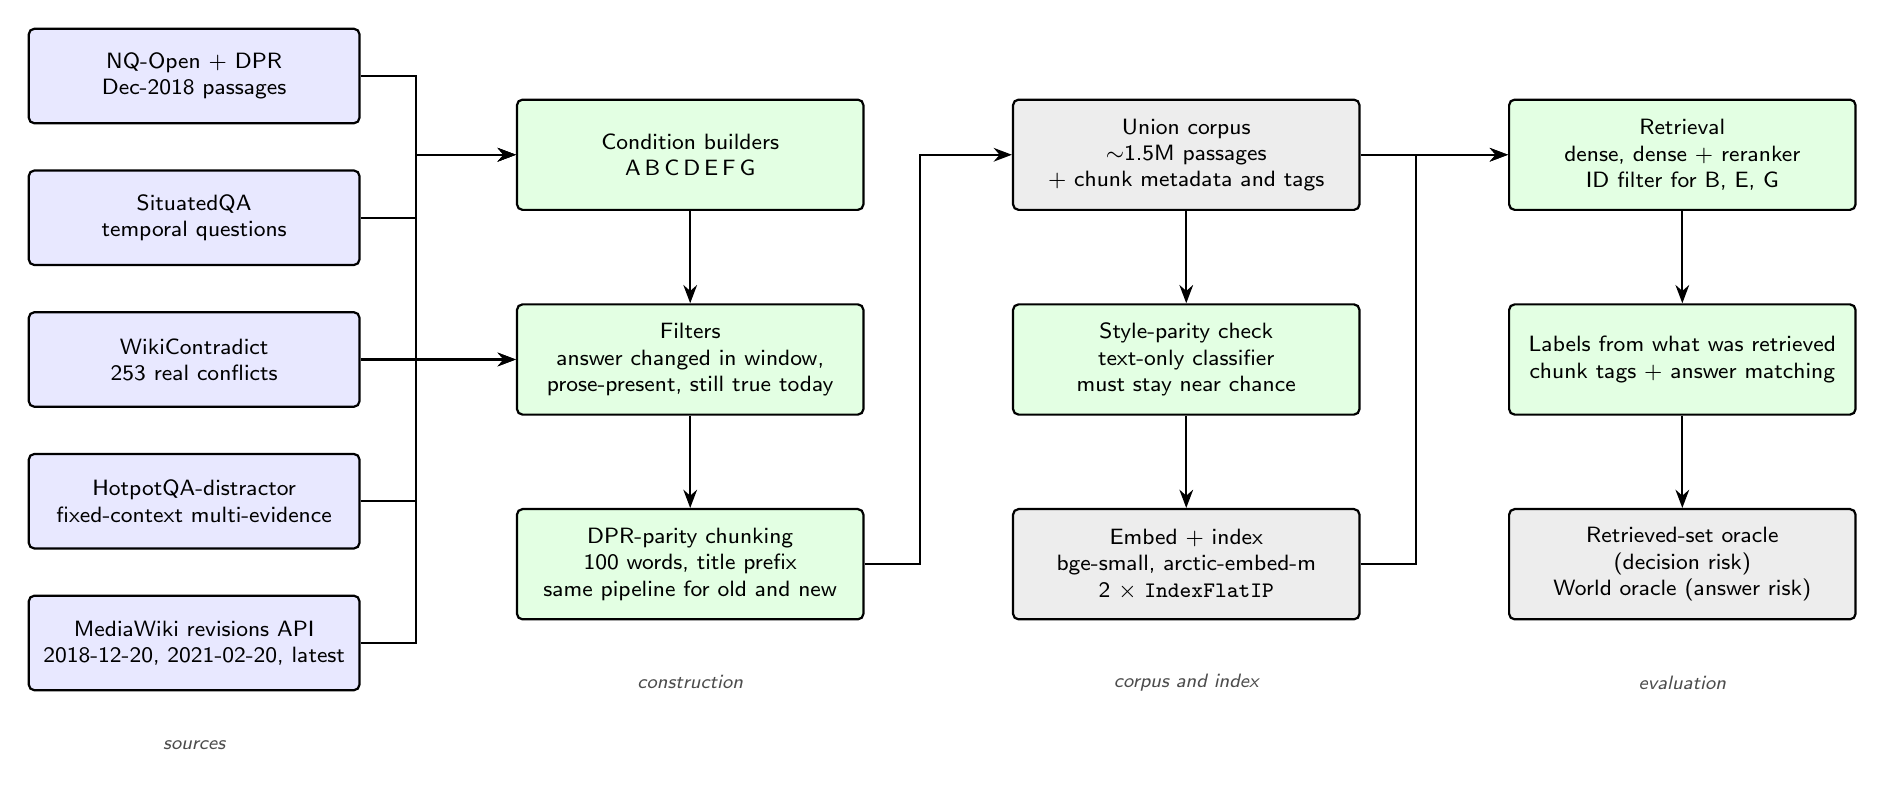
\begin{tikzpicture}[font=\sffamily\footnotesize,>=Stealth,
  box/.style={draw=black,rounded corners=2pt,thick,align=center,inner sep=4pt,fill=white},
  src/.style={box,fill=blue!9,minimum width=4.2cm,minimum height=1.2cm},
  proc/.style={box,fill=green!11,minimum width=4.4cm,minimum height=1.4cm},
  store/.style={box,fill=black!7,minimum width=4.4cm,minimum height=1.4cm},
  arr/.style={->,thick},
  lbl/.style={font=\sffamily\scriptsize\itshape,black!70}]
% sources
\node[src] (nq) at (0,4.6) {NQ-Open + DPR\\Dec-2018 passages};
\node[src] (sq) at (0,2.8) {SituatedQA\\temporal questions};
\node[src] (wc) at (0,1.0) {WikiContradict\\253 real conflicts};
\node[src] (hp) at (0,-0.8) {HotpotQA-distractor\\fixed-context multi-evidence};
\node[src] (mw) at (0,-2.6) {MediaWiki revisions API\\2018-12-20, 2021-02-20, latest};
% construction
\node[proc] (cb) at (6.3,3.6) {Condition builders\\A\,B\,C\,D\,E\,F\,G};
\node[proc] (fl) at (6.3,1.0) {Filters\\answer changed in window,\\prose-present, still true today};
\node[proc] (ck) at (6.3,-1.6) {DPR-parity chunking\\100 words, title prefix\\same pipeline for old and new};
\node[store] (uc) at (12.6,3.6) {Union corpus\\$\sim$1.5M passages\\+ chunk metadata and tags};
\node[proc] (pc) at (12.6,1.0) {Style-parity check\\text-only classifier\\must stay near chance};
\node[store] (ix) at (12.6,-1.6) {Embed + index\\bge-small, arctic-embed-m\\2 $\times$ \texttt{IndexFlatIP}};
\node[proc] (rt) at (18.9,3.6) {Retrieval\\dense, dense + reranker\\ID filter for B, E, G};
\node[proc] (lb) at (18.9,1.0) {Labels from what was retrieved\\chunk tags + answer matching};
\node[store] (or) at (18.9,-1.6) {Retrieved-set oracle\\(decision risk)\\World oracle (answer risk)};
\draw[arr] (nq.east) -- ++(0.7,0) |- (cb.west);
\draw[arr] (sq.east) -- ++(0.7,0) |- (cb.west);
\draw[arr] (wc.east) -- ++(0.7,0) |- (cb.west);
\draw[arr] (hp.east) -- ++(0.7,0) |- (fl.west);
\draw[arr] (mw.east) -- ++(0.7,0) |- (fl.west);
\draw[arr] (cb) -- (fl);
\draw[arr] (fl) -- (ck);
\draw[arr] (ck.east) -- ++(0.7,0) |- (uc.west);
\draw[arr] (uc) -- (pc);
\draw[arr] (pc) -- (ix);
\draw[arr] (uc.east) -- ++(0.7,0) |- (rt.west);
\draw[arr] (ix.east) -- ++(0.7,0) |- (rt.west);
\draw[arr] (rt) -- (lb);
\draw[arr] (lb) -- (or);
\node[lbl] at (0,-3.9) {sources};
\node[lbl] at (6.3,-3.1) {construction};
\node[lbl] at (12.6,-3.1) {corpus and index};
\node[lbl] at (18.9,-3.1) {evaluation};
\end{tikzpicture}}\\[4pt]
{\setstretch{1}\small\itshape Figure 5.2: Data, corpus-construction and labelling pipeline.}
\end{figure}


\bluesub{5.3 Proposed Algorithm / Model}
\textbf{Problem formulation.} Let $q$ be a query, $C=\{c_1,\dots,c_K\}$ the $K{=}10$ retrieved chunks, and $M=\{(d_i,t_i)\}$ their metadata, where $d_i$ is the document identifier and $t_i$ the revision timestamp. The generator emits a draft $(a,h)$, consisting of a short answer $a$ and a declarative statement $h$, together with a no-context prior answer $a_0$. The gate is a map $G(q,C,M,a,h,a_0)\rightarrow\{\text{release},\text{resolve},\text{abstain}\}$. Let $y\in\{\text{release},\text{abstain}\}$ be the retrieved-set oracle label of a draft. For released drafts, the quantities of interest are the coverage $\Phi(\tau)=\Pr[\text{released}]$ and the decision risk $R(\tau)=\Pr[y=\text{abstain}\mid\text{released}]$, where $\tau=(\tau_1,\tau_2)$ are the per-axis thresholds. The objective is to maximise $\Phi$ subject to $R\le\alpha$.

\textbf{Axis 1: answerability.} Each chunk is extended to sentence boundaries to give a premise $\bar c_i$, and a cross-encoder verifier $f_{\theta_1}$ scores the pair $(\bar c_i,h)$. Premises stay chunk-sized because chunk-level premises outperform sentence-level and document-level ones~[11]. For a bag of $K$ pair embeddings $e_i=f_{\theta_1}(\bar c_i,h)$, the pooled representation concatenates the mean and the maximum, and a head $g_1$ maps it, together with retrieval-score scalars $r$, to $s_1=\Pr[\text{sufficient}]$:
\begin{equation}
s_1 = g_1\big(\big[\,\tfrac{1}{K}\textstyle\sum_{i} e_i \;;\; \max_i e_i \;;\; r\,\big]\big).
\end{equation}
Max pooling is the natural baseline in the multiple-instance setting, because conflict and support are ``any instance'' properties of a bag. This axis reuses established machinery~[10],~[11] and is not claimed as novel. Its three aggregation levels (single-hop maximum, multi-evidence concatenation, and conflict) are reported separately.

\textbf{Axis 2: evidence reliability.} Four signals feed this axis (Figure~5.3):
\begin{itemize}
\item \emph{Inter-chunk contradiction:} for each of the top five chunks, its two most query-relevant title-prefixed sentences $\sigma$ are tested as hypotheses against every other top-five chunk as premise. Agreement is counted only across distinct documents, and identical text across revisions of one document collapses into one result after filtering. The contradiction score is
\begin{equation}
\kappa=\max_{i\neq j,\;d_i\neq d_j}\;\max_{\sigma\in S(c_i)}\;p_{\mathrm{con}}(\bar c_j,\sigma).
\end{equation}
\item \emph{Parametric divergence (CDD-lite):} $\delta=1-\mathrm{F1}(a,a_0)$, a one-sided risk flag raised when the context pulls the answer away from the model's prior. Agreement is never treated as evidence of reliability.
\item \emph{Entailment-score dispersion:} $\varsigma=\operatorname{std}_i\,p_{\mathrm{ent}}(\bar c_i,h)$, treated as a hypothesis and tested by ablation.
\item \emph{Version metadata:} $\rho=\mathbf{1}[\exists\, i,j:\; d_i=d_j,\; t_i\neq t_j]$, which fires when two retrieved chunks are different revisions of one document. Metadata is restricted to $(d_i,t_i)$. There is no ``newer version exists'' flag, because the system can only know what it can reach.
\end{itemize}
A second head $g_2$ maps the pooled pair embeddings and the scalars $(\kappa,\delta,\varsigma,\rho,r)$ to $s_2=\Pr[\text{reliable}]$ and the labels reliable, conflicting or potentially misleading. ``Reliable'' means no conflict was detected, not that the evidence is true. This is a stated epistemic limit: two mutually consistent wrong passages are indistinguishable from two consistent right ones.

\begin{figure}[t]
\centering
\resizebox{\linewidth}{!}{%
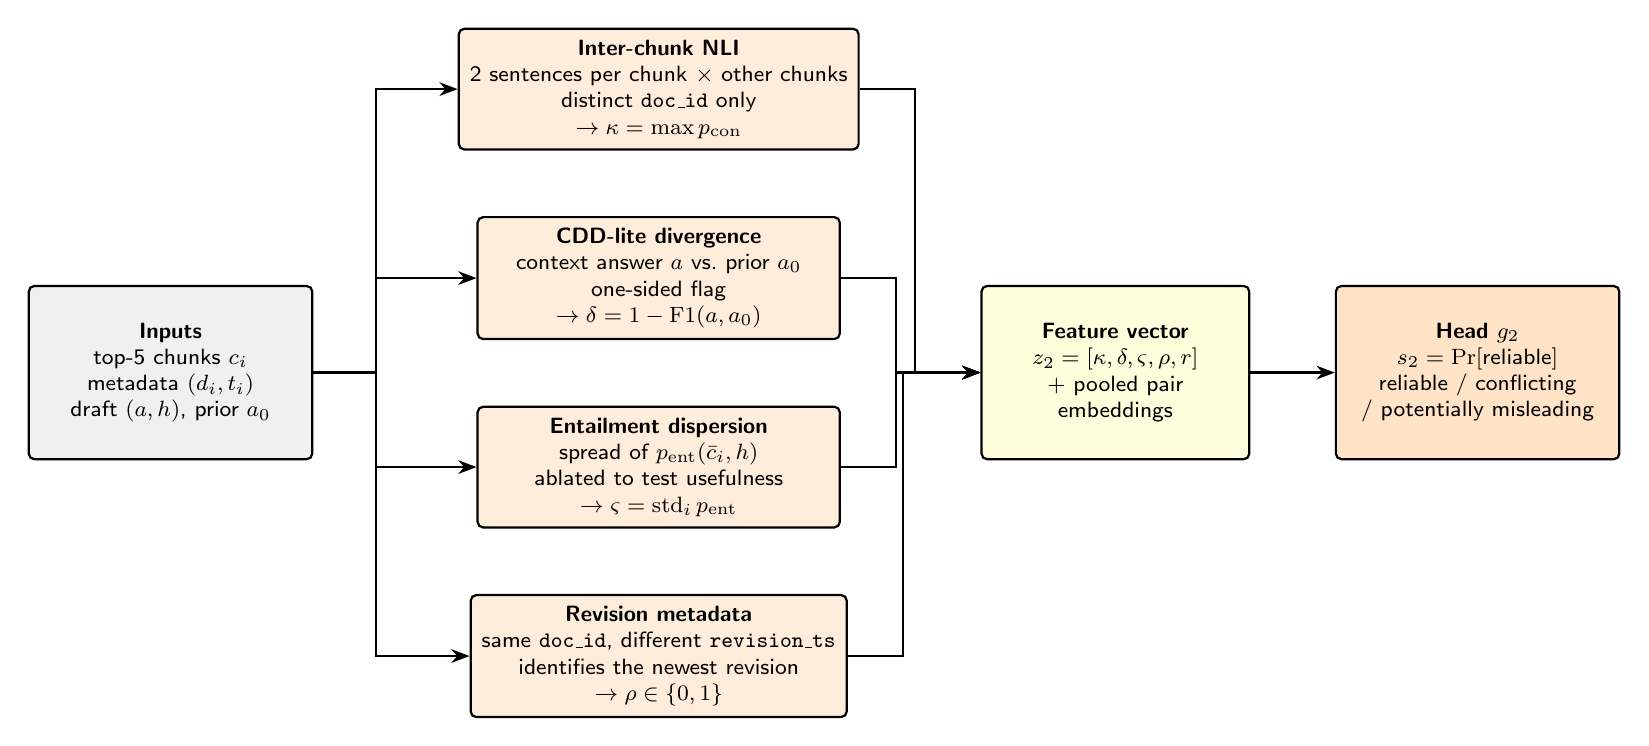
\begin{tikzpicture}[font=\sffamily\footnotesize,>=Stealth,
  box/.style={draw=black,rounded corners=2pt,thick,align=center,inner sep=4pt,fill=white},
  sig/.style={box,fill=orange!14,minimum width=4.6cm,minimum height=1.5cm},
  io/.style={box,fill=black!6},
  arr/.style={->,thick}]
\node[io,minimum width=3.6cm,minimum height=2.2cm] (in) at (0,0) {\textbf{Inputs}\\top-5 chunks $c_i$\\metadata $(d_i,t_i)$\\draft $(a,h)$, prior $a_0$};
\node[sig] (s1) at (6.2,3.6) {\textbf{Inter-chunk NLI}\\2 sentences per chunk $\times$ other chunks\\distinct \texttt{doc\_id} only\\$\rightarrow\kappa=\max p_{\mathrm{con}}$};
\node[sig] (s2) at (6.2,1.2) {\textbf{CDD-lite divergence}\\context answer $a$ vs.\ prior $a_0$\\one-sided flag\\$\rightarrow\delta=1-\mathrm{F1}(a,a_0)$};
\node[sig] (s3) at (6.2,-1.2) {\textbf{Entailment dispersion}\\spread of $p_{\mathrm{ent}}(\bar c_i,h)$\\ablated to test usefulness\\$\rightarrow\varsigma=\mathrm{std}_i\,p_{\mathrm{ent}}$};
\node[sig] (s4) at (6.2,-3.6) {\textbf{Revision metadata}\\same \texttt{doc\_id}, different \texttt{revision\_ts}\\identifies the newest revision\\$\rightarrow\rho\in\{0,1\}$};
\node[box,fill=yellow!14,minimum width=3.4cm,minimum height=2.2cm] (fv) at (12.0,0) {\textbf{Feature vector}\\$z_2=[\kappa,\delta,\varsigma,\rho,r]$\\+ pooled pair\\embeddings};
\node[box,fill=orange!22,minimum width=3.6cm,minimum height=2.2cm] (hd) at (16.6,0) {\textbf{Head $g_2$}\\$s_2=\Pr[\text{reliable}]$\\reliable $/$ conflicting\\$/$ potentially misleading};
\foreach \y in {s1,s2,s3,s4}{\draw[arr] (in.east) -- ++(0.8,0) |- (\y.west);}
\foreach \y in {s1,s2,s3,s4}{\draw[arr] (\y.east) -- ++(0.7,0) |- (fv.west);}
\draw[arr] (fv) -- (hd);
\end{tikzpicture}}\\[4pt]
{\setstretch{1}\small\itshape Figure 5.3: Internal structure of the Axis-2 evidence-reliability module.}
\end{figure}

\textbf{Decision rule.} The decision table (Table~5.2) is fixed, not learned. Formally, a draft is released if $s_1\ge\tau_1$ and $s_2\ge\tau_2$. It is resolved if $s_1\ge\tau_1$ and the conflict lies between revisions of one document ($\rho=1$). In every other case the gate abstains. A conflict between different documents always abstains.
\par\nopagebreak\noindent{\setstretch{1}\small\bfseries Table 5.2: Decision table}\par\nopagebreak\vspace{2pt}
\renewcommand{\arraystretch}{1.4}
\begin{longtable}{|>{\raggedright\arraybackslash\setlength{\parskip}{0pt}\setstretch{1}\small}p{0.20\linewidth}|>{\raggedright\arraybackslash\setlength{\parskip}{0pt}\setstretch{1}\small}p{0.33\linewidth}|>{\raggedright\arraybackslash\setlength{\parskip}{0pt}\setstretch{1}\small}p{0.37\linewidth}|}
\hline
\rowcolor{ghead}\bfseries Axis 1 & \bfseries Axis 2 & \bfseries Decision \\ \hline
Insufficient / uncertain & not evaluated & Abstain \\ \hline
Sufficient & Reliable & Release the draft with a citation \\ \hline
Sufficient & Conflicting, between revisions of one document & Regenerate from the newest revision, re-check Axis 1, release or abstain \\ \hline
Sufficient & Conflicting, between different documents & Abstain \\ \hline
Sufficient & Potentially misleading & Abstain \\ \hline
\end{longtable}

\textbf{Gate variants.} Both variants read the same bags of verifier pairs (10 statement--chunk pairs for Axis 1 and about 40 sentence--chunk pairs for Axis 2) plus shared scalar features (Figure~5.4). No variant feeds all chunks through one encoder as a single sequence, because ten 100-word chunks already exceed a 512-token window.
\begin{itemize}
\item \emph{Variant A (two-axis):} two separate fine-tuned verifier encoders, one per axis, each pooling its pair embeddings by mean and max before its own head. No weights are shared, so Axis 1 cannot absorb reliability signals.
\item \emph{Variant C (single classifier):} frozen off-the-shelf verifier outputs, pooled per bag, plus the scalar features, fed to one four-way logistic-regression or gradient-boosted classifier trained on CPU.
\end{itemize}
Variants A and C differ in both axis separation and fine-tuning, so a gap between them is first checked with a cheap control: the same frozen features with two separate per-axis classifiers. A stretch variant B (one shared encoder, two heads) completes the separation ladder from fully separate (A), through shared representation with separate outputs (B), to fully combined (C). Attention-based pooling~[18] is run only as a sensitivity check if A trails C.

\begin{figure}[t]
\centering
\resizebox{\linewidth}{!}{%
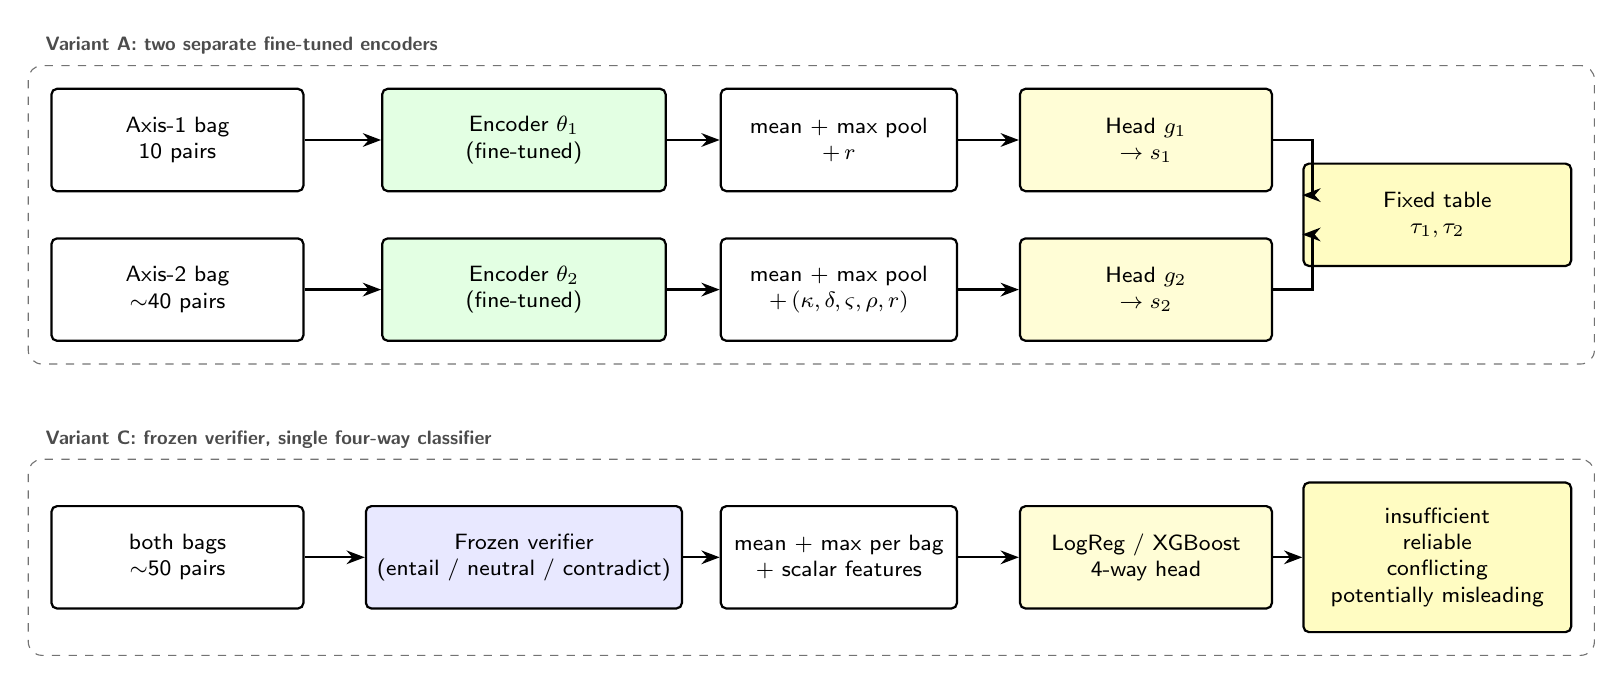
\begin{tikzpicture}[font=\sffamily\footnotesize,>=Stealth,
  box/.style={draw=black,rounded corners=2pt,thick,align=center,inner sep=4pt,fill=white},
  enc/.style={box,fill=green!11,minimum width=3.6cm,minimum height=1.3cm},
  frz/.style={box,fill=blue!9,minimum width=3.6cm,minimum height=1.3cm},
  hd/.style={box,fill=yellow!16,minimum width=3.2cm,minimum height=1.3cm},
  arr/.style={->,thick},
  lbl/.style={font=\sffamily\scriptsize\itshape,black!70}]
% Variant A
\node[lbl,anchor=west] at (-0.2,3.1) {\textbf{Variant A: two separate fine-tuned encoders}};
\node[box,minimum width=3.2cm,minimum height=1.3cm] (a1b) at (1.6,1.9) {Axis-1 bag\\10 pairs};
\node[enc] (a1e) at (6.0,1.9) {Encoder $\theta_1$\\(fine-tuned)};
\node[box,minimum width=3.0cm,minimum height=1.3cm] (a1p) at (10.0,1.9) {mean + max pool\\$+\,r$};
\node[hd] (a1h) at (13.9,1.9) {Head $g_1$\\$\rightarrow s_1$};
\node[box,minimum width=3.2cm,minimum height=1.3cm] (a2b) at (1.6,0) {Axis-2 bag\\$\sim$40 pairs};
\node[enc] (a2e) at (6.0,0) {Encoder $\theta_2$\\(fine-tuned)};
\node[box,minimum width=3.0cm,minimum height=1.3cm] (a2p) at (10.0,0) {mean + max pool\\$+\,(\kappa,\delta,\varsigma,\rho,r)$};
\node[hd] (a2h) at (13.9,0) {Head $g_2$\\$\rightarrow s_2$};
\draw[arr] (a1b)--(a1e); \draw[arr] (a1e)--(a1p); \draw[arr] (a1p)--(a1h);
\draw[arr] (a2b)--(a2e); \draw[arr] (a2e)--(a2p); \draw[arr] (a2p)--(a2h);
\node[box,fill=yellow!24,minimum width=3.4cm,minimum height=1.3cm] (ad) at (17.6,0.95) {Fixed table\\$\tau_1,\tau_2$};
\draw[arr] (a1h.east) -- ++(0.5,0) |- ([yshift=0.25cm]ad.west);
\draw[arr] (a2h.east) -- ++(0.5,0) |- ([yshift=-0.25cm]ad.west);
% Variant C
\node[lbl,anchor=west] at (-0.2,-1.9) {\textbf{Variant C: frozen verifier, single four-way classifier}};
\node[box,minimum width=3.2cm,minimum height=1.3cm] (cb) at (1.6,-3.4) {both bags\\$\sim$50 pairs};
\node[frz] (cv) at (6.0,-3.4) {Frozen verifier\\(entail / neutral / contradict)};
\node[box,minimum width=3.0cm,minimum height=1.3cm] (cp) at (10.0,-3.4) {mean + max per bag\\$+$ scalar features};
\node[hd,minimum width=3.2cm] (ch) at (13.9,-3.4) {LogReg / XGBoost\\4-way head};
\node[box,fill=yellow!24,minimum width=3.4cm,minimum height=1.9cm] (cd) at (17.6,-3.4) {insufficient\\reliable\\conflicting\\potentially misleading};
\draw[arr] (cb)--(cv); \draw[arr] (cv)--(cp); \draw[arr] (cp)--(ch); \draw[arr] (ch)--(cd);
\begin{scope}[on background layer]
\node[draw=black!55,dashed,rounded corners=5pt,inner sep=8pt,fit=(a1b)(a2b)(ad)(a1h)(a2h)] {};
\node[draw=black!55,dashed,rounded corners=5pt,inner sep=8pt,fit=(cb)(cd)(cv)(ch)] {};
\end{scope}
\end{tikzpicture}}\\[4pt]
{\setstretch{1}\small\itshape Figure 5.4: Gate variants A (separate fine-tuned encoders) and C (frozen features, single classifier).}
\end{figure}

\textbf{Planned training settings (to be tuned on the dev split).} Variant A fine-tunes each encoder with cross-entropy loss and the AdamW optimiser, a learning rate near $2\times10^{-5}$, batch size 16 and about two epochs, with Axis-2 bags capped at 20 pairs during training. Each pooled vector is concatenated with the scalar features and passed to a small multilayer-perceptron head. Variant C uses logistic regression or XGBoost with regularisation chosen by cross-validation on dev. The verifier backbone is chosen in the go/no-go check from three candidates (a 0.1B NLI cross-encoder, AlignScore-base and MiniCheck at 355M) by accuracy per unit of latency.

\textbf{Calibration and risk control.} Each axis is calibrated independently on the dev split by temperature scaling, $\hat p=\mathrm{softmax}(z/T)$ with $T$ fitted by negative log-likelihood, and calibration is reported as expected calibration error over 15 equal-width bins, Brier score and reliability diagrams. Thresholds are then chosen by confidence-interval risk control~[8]: the largest coverage whose Clopper--Pearson upper bound on decision risk stays below a target $\alpha$ (for example 2\%) at confidence $1-\delta=0.95$. Sweeping $\tau_1$ and $\tau_2$ gives a two-dimensional risk--coverage surface.

\textbf{Retrieval.} Exact cosine search (FAISS \texttt{IndexFlatIP}) is used rather than approximate search, because the study needs to know exactly whether a passage reached the top 10. Conditions B, E and G hide passages at query time by ID filtering, which returns the same top 10 as deleting them. Two embedding models are used (bge-small as the default and arctic-embed-m for robustness), each indexing the full corpus. A second retrieval arm reranks the dense top 100 with a cross-encoder to test whether reranking removes misleading passages on its own.

\textbf{Cost model.} Per query, the gate adds about 50 verifier pair evaluations, batched, and one short parallel generation for CDD-lite. Deployment may skip Axis 2 once Axis 1 reports insufficient support, which saves cost without changing the decision. Cost is reported with and without CDD-lite, since it is the only language-model call inside the gate.

\textbf{Baselines.} Table~5.3 lists the five baselines. Every method receives the same query, retrieved chunks with metadata, and draft, and makes the same release-or-abstain decision. Judges may also choose ``answer from the newer revision'', so that condition D is compared fairly.
\par\nopagebreak\noindent{\setstretch{1}\small\bfseries Table 5.3: Baseline methods}\par\nopagebreak\vspace{2pt}
\renewcommand{\arraystretch}{1.4}
\begin{longtable}{|>{\centering\arraybackslash\setlength{\parskip}{0pt}\setstretch{1}\small}p{0.06\linewidth}|>{\raggedright\arraybackslash\setlength{\parskip}{0pt}\setstretch{1}\small}p{0.30\linewidth}|>{\raggedright\arraybackslash\setlength{\parskip}{0pt}\setstretch{1}\small}p{0.50\linewidth}|}
\hline
\rowcolor{ghead}\bfseries No. & \bfseries Method & \bfseries Role \\ \hline
1 & Retrieval-score threshold & Uses retrieval scores only; the cheapest possible gate \\ \hline
2 & Zero-shot verifier & Single-axis control: the untrained verifier checks the draft statement (Axis 1 only) \\ \hline
3 & Set-level verifier (SURE-RAG-style) & Closest cheap prior art~[4]; reimplemented because its code is not released \\ \hline
4 & Cheap LLM judge & Reads the full context; labels both axes \\ \hline
5 & Strong LLM judge & Upper reference on cost and accuracy; test split only \\ \hline
\end{longtable}

\textbf{What is novel and what is adopted.} Claim verification, small verifiers matching large models, and the separation of answerability from correctness are adopted from prior work~[7], [10], [11]. We do not claim novelty for them. The contribution is narrower: explicit two-axis gating with independent calibration, passage--passage reasoning across retrieved chunks, temporal conditions with a metadata ablation, and realistic retrieval with measured survival of misleading passages.

\bluesub{5.4 Implementation Plan (Phase-wise)}
\par\nopagebreak\noindent{\setstretch{1}\small\bfseries Table 5.4: Implementation plan}\par\nopagebreak\vspace{2pt}
\renewcommand{\arraystretch}{1.4}
\begin{longtable}{|>{\centering\arraybackslash\setlength{\parskip}{0pt}\setstretch{1}\small}p{0.07\linewidth}|>{\raggedright\arraybackslash\setlength{\parskip}{0pt}\setstretch{1}\small}p{0.26\linewidth}|>{\raggedright\arraybackslash\setlength{\parskip}{0pt}\setstretch{1}\small}p{0.43\linewidth}|>{\raggedright\arraybackslash\setlength{\parskip}{0pt}\setstretch{1}\small}p{0.11\linewidth}|}
\hline
\rowcolor{ghead}\bfseries Phase & \bfseries Task to be completed & \bfseries Activities involved & \bfseries Duration \\ \hline
I & Literature Review \& Problem Definition & Survey related work, finalise research questions, scope and non-goals & 2 weeks \\ \hline
II & Dataset Acquisition \& Pre-processing & Count the stale-question yield first; build conditions A--G, the 1.5M-passage corpus and two FAISS indices; run the style-parity check; hand-verify samples & 3 weeks \\ \hline
III & System Design \& Phase 0 Check & Design the pipeline; run the 100-example go/no-go; choose the verifier backbone; check draft format & 2 weeks \\ \hline
IV & Implementation \& Training & Build both gate variants and the set-level verifier baseline; fine-tune and calibrate on the dev split & 5 weeks \\ \hline
V & Evaluation \& Testing & Run the core grid, ablations, embedding-robustness runs and post-release scoring & 3 weeks \\ \hline
VI & Documentation \& Reporting & Final report, paper draft, presentation & 3 weeks \\ \hline
\end{longtable}

\Needspace{9\baselineskip}
\bluesub{5.5 Tools \& Technologies}
\par\nopagebreak\noindent{\setstretch{1}\small\bfseries Table 5.5: Tools and technologies}\par\nopagebreak\vspace{2pt}
\renewcommand{\arraystretch}{1.6}
\begin{longtable}{|>{\raggedright\arraybackslash\setlength{\parskip}{0pt}\setstretch{1}\bfseries}p{0.30\linewidth}|>{\raggedright\arraybackslash\setlength{\parskip}{0pt}\setstretch{1}\small}p{0.60\linewidth}|}
\hline
\rowcolor{ghead}\bfseries Category & \bfseries\color{black}\normalsize Tools / Technologies / Versions \\* \hline
Programming Language & Python 3.11 or later (pinned in \texttt{.python-version} and \texttt{pyproject.toml}) \\ \hline
Frameworks / Libraries & PyTorch, Hugging Face Transformers, sentence-transformers, FAISS, vLLM, scikit-learn, XGBoost, Hydra, Pydantic, RAGAS, litellm \\ \hline
Development Environment & Linux laptop workstation with an NVIDIA RTX 4070 Laptop GPU (8 GB); VS Code as the editor with the integrated terminal; \texttt{uv} for virtual environments, dependency resolution and a locked \texttt{uv.lock} file; \texttt{src/} package layout with library code kept free of disk side effects; Hydra configuration files for each grid cell; numbered stage scripts that read a config and write an artifact, with skip-if-exists checks; \texttt{pytest} unit and end-to-end smoke tests on a tiny fixture corpus; Jupyter notebooks for exploratory analysis and plotting; Claude Code (an AI coding assistant) for scaffolding and review, with all results and decisions checked by the authors \\ \hline
Database / Storage & JSON Lines files for chunks and questions; FAISS indices (about 7 GB for two models) on local disk \\ \hline
Hardware / Platform & Laptop: Intel Core i9-14900HX (24 cores, 32 threads), NVIDIA GeForce RTX 4070 Laptop GPU (8 GB GDDR6), 32 GB DDR5-5600 RAM, PCIe 4.0 NVMe SSD. The 8B generator runs 4-bit quantised to fit the 8 GB GPU, which is disclosed as a deviation from unquantised settings \\ \hline
Version Control & Git \\ \hline
Other Tools & MediaWiki revisions API for article revisions; hosted LLM APIs for the two judges \\ \hline
\end{longtable}

\Needspace{12\baselineskip}
\bluesub{5.6 Risk Analysis and Mitigation}
\par\nopagebreak\noindent{\setstretch{1}\small\bfseries Table 5.6: Project risks and mitigation}\par\nopagebreak\vspace{2pt}
\renewcommand{\arraystretch}{1.4}
\begin{longtable}{|>{\raggedright\arraybackslash\setlength{\parskip}{0pt}\setstretch{1}\small\bfseries}p{0.30\linewidth}|>{\raggedright\arraybackslash\setlength{\parskip}{0pt}\setstretch{1}\small}p{0.60\linewidth}|}
\hline
\rowcolor{ghead}\bfseries Risk & \bfseries Mitigation \\ \hline
Few stale-question items survive the three filters (answer changed, prose-present, still true today) & Count the yield first, in the data phase; if too small, bring forward the five-snapshot TemporalWiki probes \\ \hline
Constructed chunks look different from original ones, leaking the label & Replicate the original chunking exactly; run the text-only style-parity classifier and rebuild any text that fails \\ \hline
String-matching labels count coincidental mentions & Hand-verify a sample per condition and report the estimated label noise \\ \hline
Generator knowledge is newer than the corpus (December 2023 against February 2021) & Keep only items whose gold answer is also true in the latest revision \\ \hline
Malformed drafts (missing statement, or statement and answer disagree) & Measure the rate in the go/no-go check; withheld drafts are counted as lost coverage \\ \hline
Compute limits of an 8 GB laptop GPU & Exact search at 1.5M passages, features computed once and shared across variants, 4-bit quantised generator with reduced batch sizes, disclosed as a deviation \\ \hline
Judge and evaluator model versions change over time & Pin versions at implementation time and use a RAGAS model different from both judges \\ \hline
\end{longtable}

\redsec{6. Expected Outcomes \& Deliverables}
\dredrule
Upon successful completion of this project, the following outcomes are expected:

\purpsub{6.1 Technical Outcomes}
\begin{itemize}
\item\relax A working draft--verify--release pipeline with two calibrated gate variants and five baselines, run over 58 core grid cells (about 83 configurations with ablations).
\item\relax Target: at least 10$\times$ lower per-query latency and cost than the strong LLM judge, at a decision risk within a few points of the cheap judge. These are targets, and a miss is also a reportable result.
\item\relax Target: expected calibration error below 0.05 for each axis on the test split.
\item\relax Risk--coverage curves for decision risk and answer risk on each of the seven evidence conditions, with error rate at 80\% coverage and maximum coverage at 2\% risk reported as operating points.
\item\relax Per-query latency and cost for every method, so the gate can be compared with the judges on cost as well as accuracy.
\item\relax A measurement of how much version metadata adds, and how many false abstentions it costs on old-but-valid evidence.
\end{itemize}

\purpsub{6.2 Research Outcomes}
\begin{itemize}
\item\relax A reportable answer, positive or negative, to each of five research questions: gate versus judges, two axes versus one, natural versus synthetic conflicts, the value of metadata, and whether reranking alone filters misleading passages.
\item\relax A paper draft for submission to an NLP or information-retrieval venue.
\end{itemize}

\purpsub{6.3 Deliverables Checklist}
\par\nopagebreak\noindent{\setstretch{1}\small\bfseries Table 6.1: Deliverables and target timeline}\par\nopagebreak\vspace{2pt}
\renewcommand{\arraystretch}{1.5}
\begin{longtable}{|>{\raggedright\arraybackslash\setlength{\parskip}{0pt}\setstretch{1}\small}p{0.55\linewidth}|>{\raggedright\arraybackslash\setlength{\parskip}{0pt}\setstretch{1}\small}p{0.345\linewidth}|}
\hline
\rowcolor{ghead}\bfseries Deliverable & \bfseries Target Timeline \\ \hline
Synopsis / Proposal Document & Week 1 \\ \hline
Literature Review Report & Week 2 \\ \hline
Working Prototype / Baseline Model & Week 7 \\ \hline
Final Trained Model + Code Repository & Week 12 \\ \hline
Evaluation Report \& Results & Week 15 \\ \hline
Journal / Conference Paper Draft & Week 17 \\ \hline
Final Project Report \& Presentation & Week 18 \\ \hline
\end{longtable}

\purpsec{7. Evaluation Metrics \& Validation Plan}
\dredrule
\textbf{Metrics:}
\begin{itemize}
\item\relax \emph{Gate quality:} coverage (fraction of drafts released); decision risk (released drafts the retrieved-set oracle says to withhold); answer risk (released answers wrong against the world oracle); abstention precision and recall.
\item\relax \emph{Curves and operating points:} risk--coverage curves per condition and variant~[14], with thresholds chosen under a risk-control rule~[8].
\item\relax \emph{Calibration:} expected calibration error, Brier score and reliability diagrams for each axis and variant.
\item\relax \emph{Retrieval control:} precision, recall, MRR and nDCG at 10, and the fraction of misleading passages that survive to the top 10.
\item\relax \emph{Post-release check:} RAGAS faithfulness, answer relevancy and correctness on released answers only. These never tune the gate. BLEU, ROUGE and perplexity are excluded because they score word overlap and cannot evaluate an abstain decision.
\end{itemize}

\textbf{Experimental matrix and compute.} The core grid crosses seven evidence conditions with seven methods (variants A and C plus five baselines) on dense-only retrieval, giving 49 cells. The reranked arm adds conditions C, D and F with three methods (A, C and the cheap judge), giving 9 cells, so the core grid is 58 cells. Secondary runs bring the total to about 83 configurations (Table~7.1). Compute is estimated at 9--22 GPU-hours on a single GPU (Table~7.2), to be rechecked in the go/no-go check.
\par\nopagebreak\noindent{\setstretch{1}\small\bfseries Table 7.1: Experimental matrix}\par\nopagebreak\vspace{2pt}
\renewcommand{\arraystretch}{1.4}
\begin{longtable}{|>{\raggedright\arraybackslash\setlength{\parskip}{0pt}\setstretch{1}\small\bfseries}p{0.30\linewidth}|>{\raggedright\arraybackslash\setlength{\parskip}{0pt}\setstretch{1}\small}p{0.50\linewidth}|>{\centering\arraybackslash\setlength{\parskip}{0pt}\setstretch{1}\small}p{0.10\linewidth}|}
\hline
\rowcolor{ghead}\bfseries Run & \bfseries Scope & \bfseries Cells \\ \hline
Core, dense-only & 7 conditions $\times$ 7 methods & 49 \\ \hline
Core, reranked & Conditions C, D, F $\times$ 3 methods & 9 \\ \hline
Embedding robustness & Second embedding model, conditions D and F, best variant & 2 \\ \hline
Metadata-off ablation & Best variant retrained without metadata, 7 conditions & 7 \\ \hline
Divergence-off ablation & Best variant retrained without CDD-lite, 7 conditions & 7 \\ \hline
Dispersion-off ablation & Best variant retrained without dispersion, 7 conditions & 7 \\ \hline
Always-abstain on D & Decision-table change only, condition D, 2 retrieval arms & 2 \\ \hline
\bfseries Total & Plus a separate multi-evidence table on HotpotQA-distractor & \bfseries 83 \\ \hline
\end{longtable}
\par\nopagebreak\noindent{\setstretch{1}\small\bfseries Table 7.2: Estimated compute budget (single laptop GPU)}\par\nopagebreak\vspace{2pt}
\renewcommand{\arraystretch}{1.4}
\begin{longtable}{|>{\raggedright\arraybackslash\setlength{\parskip}{0pt}\setstretch{1}\small\bfseries}p{0.50\linewidth}|>{\raggedright\arraybackslash\setlength{\parskip}{0pt}\setstretch{1}\small}p{0.40\linewidth}|}
\hline
\rowcolor{ghead}\bfseries Stage & \bfseries Estimate \\ \hline
Embed 1.5M passages with two models & 1--2 GPU-hours \\ \hline
Rerank dense top-100 for all conditions & 2--3 GPU-hours \\ \hline
Verification, about 1.5M pairs & 0.75 GPU-hours (0.1B) to 2 (355M) \\ \hline
Generation, about 45k short outputs with vLLM & 1--1.5 GPU-hours \\ \hline
Gate training and ablation retraining & 3--9 GPU-hours (A); minutes on CPU (C) \\ \hline
\bfseries Total & \bfseries 9--22 GPU-hours \\ \hline
\end{longtable}

These figures are order-of-magnitude estimates. They will be re-measured on the RTX 4070 Laptop GPU in the go/no-go check, where the 8 GB memory limit means smaller batches and a 4-bit generator.

\textbf{Statistical analysis.} Uncertainty is reported as bootstrap 95\% confidence intervals over questions (1,000 resamples), and differences between methods are tested with a paired bootstrap on identical drafts. Because the go/no-go sample has only 20 items per condition, intervals there are roughly $\pm$20 points, so only large gaps are acted on. Selective-prediction curves follow the standard risk--coverage protocol~[14],~[15].

\textbf{Validation Strategy:}
\begin{itemize}
\item\relax Splits are by question: no question appears in more than one of train, dev and test.
\item\relax A 100-example go/no-go check (20 each from A, B, E, F and G) runs before gate training. Its confidence intervals are about $\pm$20 points, so only large gaps are acted on.
\item\relax A few hundred examples per constructed condition are hand-verified. A text-only style classifier must not tell constructed chunks from original ones, which guards against leakage through formatting.
\item\relax Ablations: metadata on or off, parametric divergence on or off, dispersion on or off, and resolve versus always-abstain on condition D. All methods are compared on the same drafts under identical conditions.
\end{itemize}

\textbf{Limitations stated in advance:}
\begin{itemize}
\item\relax The gate cannot establish that evidence is true, only inconsistency and, with metadata, revision order.
\item\relax Without a cross-family transfer test, in-distribution results cannot rule out artefacts of the editing procedure, and the report will say so.
\item\relax The reranked arm covers conditions C, D and F only.
\end{itemize}

\textbf{Ethical Considerations:}
\begin{itemize}
\item\relax All data are public (Wikipedia-derived corpora and published benchmarks); no human subjects or personal data are involved, so no ethics-board approval is needed.
\item\relax Planted false passages exist only inside the experimental corpus and are not published as facts.
\item\relax The 4-bit quantisation of the generator and the judge model versions will be disclosed as deviations or settings.
\end{itemize}

\purpsec{8. References}
\dredrule
\begingroup
\setstretch{1}\setlength{\parskip}{6pt}\sloppy\emergencystretch=3em\urlstyle{same}
\newcommand{\refitem}[1]{\par\noindent\hangindent=2.4em\hangafter=1 #1}
\vspace{4pt}
\refitem{[1]\hspace{0.5em}H. Joren, J. Zhang, C.-S. Ferng, D.-C. Juan, A. Taly, and C. Rashtchian, ``Sufficient context: A new lens on retrieval augmented generation systems,'' \textit{arXiv preprint arXiv:2411.06037}, 2024. [Online]. Available: \url{https://arxiv.org/abs/2411.06037}. \mbox{[Accessed: 03 Oct. 2026]}.}

\refitem{[2]\hspace{0.5em}Y. A. Setiawan, ``Prompt-based abstention fails under misleading context: A controlled study of small frozen RAG models,'' \textit{arXiv preprint arXiv:2608.22228}, 2026. [Online]. Available: \url{https://arxiv.org/abs/2608.22228}. \mbox{[Accessed: 03 Oct. 2026]}.}

\refitem{[3]\hspace{0.5em}Y. Chen \textit{et al.}, ``Does RAG know when retrieval is wrong? Diagnosing context compliance under knowledge conflict,'' \textit{arXiv preprint arXiv:2605.14473}, 2026. [Online]. Available: \url{https://arxiv.org/abs/2605.14473}. \mbox{[Accessed: 03 Oct. 2026]}.}

\refitem{[4]\hspace{0.5em}J. Qiu, Z. Han, and C. Huang, ``SURE-RAG: Sufficiency and uncertainty-aware evidence verification for selective retrieval-augmented generation,'' \textit{arXiv preprint arXiv:2605.03534}, 2026. [Online]. Available: \url{https://arxiv.org/abs/2605.03534}. \mbox{[Accessed: 03 Oct. 2026]}.}

\refitem{[5]\hspace{0.5em}C. Wang, Y. Li, Y. Liu, and Y. Shu, ``ConflictRAG: Detecting and resolving knowledge conflicts in retrieval augmented generation,'' \textit{arXiv preprint arXiv:2605.17301}, 2026. [Online]. Available: \url{https://arxiv.org/abs/2605.17301}. \mbox{[Accessed: 03 Oct. 2026]}.}

\refitem{[6]\hspace{0.5em}X. Zhu \textit{et al.}, ``Trust or abstain? A self-aware RAG approach,'' \textit{arXiv preprint arXiv:2605.18792}, 2026. [Online]. Available: \url{https://arxiv.org/abs/2605.18792}. \mbox{[Accessed: 03 Oct. 2026]}.}

\refitem{[7]\hspace{0.5em}B. J. Wagner, ``Two axes of LLM abstention: Answer correctness and question answerability,'' \textit{arXiv preprint arXiv:2607.08456}, 2026. [Online]. Available: \url{https://arxiv.org/abs/2607.08456}. \mbox{[Accessed: 03 Oct. 2026]}.}

\refitem{[8]\hspace{0.5em}S. Dong and H. Shinnou, ``Uncertainty-aware abstention in large language models with provable alignment guarantees,'' \textit{arXiv preprint arXiv:2607.04430}, 2026. [Online]. Available: \url{https://arxiv.org/abs/2607.04430}. \mbox{[Accessed: 03 Oct. 2026]}.}

\refitem{[9]\hspace{0.5em}Y. Hou \textit{et al.}, ``WikiContradict: A benchmark for evaluating LLMs on real-world knowledge conflicts from Wikipedia,'' \textit{arXiv preprint arXiv:2406.13805}, 2024. [Online]. Available: \url{https://arxiv.org/abs/2406.13805}. \mbox{[Accessed: 03 Oct. 2026]}.}

\refitem{[10]\hspace{0.5em}L. Tang, P. Laban, and G. Durrett, ``MiniCheck: Efficient fact-checking of LLMs on grounding documents,'' in \textit{Proc. Conf. Empirical Methods in Natural Language Processing (EMNLP)}, 2024. [Online]. Available: \url{https://arxiv.org/abs/2404.10774}. \mbox{[Accessed: 03 Oct. 2026]}.}

\refitem{[11]\hspace{0.5em}Y. Zha, Y. Yang, R. Li, and Z. Hu, ``AlignScore: Evaluating factual consistency with a unified alignment function,'' in \textit{Proc. Annu. Meeting Assoc. Comput. Linguistics (ACL)}, 2023. [Online]. Available: \url{https://arxiv.org/abs/2305.16739}. \mbox{[Accessed: 03 Oct. 2026]}.}

\refitem{[12]\hspace{0.5em}M. J. Q. Zhang and E. Choi, ``SituatedQA: Incorporating extra-linguistic contexts into QA,'' in \textit{Proc. Conf. Empirical Methods in Natural Language Processing (EMNLP)}, 2021. [Online]. Available: \url{https://arxiv.org/abs/2109.06157}. \mbox{[Accessed: 03 Oct. 2026]}.}

\refitem{[13]\hspace{0.5em}V. Karpukhin \textit{et al.}, ``Dense passage retrieval for open-domain question answering,'' in \textit{Proc. Conf. Empirical Methods in Natural Language Processing (EMNLP)}, 2020. [Online]. Available: \url{https://arxiv.org/abs/2004.04906}. \mbox{[Accessed: 03 Oct. 2026]}.}

\refitem{[14]\hspace{0.5em}R. El-Yaniv and Y. Wiener, ``On the foundations of noise-free selective classification,'' \textit{J. Mach. Learn. Res.}, vol. 11, pp. 1605--1641, 2010.}

\refitem{[15]\hspace{0.5em}Y. Geifman and R. El-Yaniv, ``Selective classification for deep neural networks,'' \textit{arXiv preprint arXiv:1705.08500}, 2017. [Online]. Available: \url{https://arxiv.org/abs/1705.08500}. \mbox{[Accessed: 03 Oct. 2026]}.}

\refitem{[16]\hspace{0.5em}P. Laban, T. Schnabel, P. N. Bennett, and M. A. Hearst, ``SummaC: Re-visiting NLI-based models for inconsistency detection in summarization,'' \textit{Trans. Assoc. Comput. Linguistics (TACL)}, 2021. [Online]. Available: \url{https://arxiv.org/abs/2111.09525}. \mbox{[Accessed: 03 Oct. 2026]}.}

\refitem{[17]\hspace{0.5em}T. Chen \textit{et al.}, ``Dense X retrieval: What retrieval granularity should we use?'' \textit{arXiv preprint arXiv:2312.06648}, 2023. [Online]. Available: \url{https://arxiv.org/abs/2312.06648}. \mbox{[Accessed: 03 Oct. 2026]}.}

\refitem{[18]\hspace{0.5em}M. Ilse, J. M. Tomczak, and M. Welling, ``Attention-based deep multiple instance learning,'' in \textit{Proc. Int. Conf. Machine Learning (ICML)}, 2018. [Online]. Available: \url{https://arxiv.org/abs/1802.04712}. \mbox{[Accessed: 03 Oct. 2026]}.}

\endgroup

\vspace{6pt}\Needspace{12\baselineskip}
\purpsec{9. Declaration \& Signatures}
\dredrule
{\itshape I/We hereby declare that this project synopsis is our original work carried out as part of the AI and ML Course. This work has not been submitted elsewhere for any other degree or examination. All sources of information have been duly cited and acknowledged.}

\vspace{6pt}
\noindent\begin{minipage}[t]{0.5\linewidth}
\setstretch{1.15}
\textbf{Student Signature:}\\[1.1cm]
\rule{0.93\linewidth}{0.5pt}\\[-2pt]
{\itshape\small\color{gtext}Snehal Reddy Thadigotla (1RV24IS126)\\ Sumukha Upadhyaya (1RV24IS130)}\\
{\itshape\small\color{gtext}Date: \rule[-2pt]{3.4cm}{0.4pt}}
\end{minipage}%
\vrule\hspace{8pt}%
\begin{minipage}[t]{0.46\linewidth}
\setstretch{1.15}
\textbf{Guide Signature:}\\[1.1cm]
\rule{\linewidth}{0.5pt}\\[-2pt]
{\itshape\small\color{gtext}Dr. Merin Meleet}\\
{\itshape\small\color{gtext}Date: \rule[-2pt]{3.4cm}{0.4pt}}
\end{minipage}

\end{document}
